\subsection{Period 2: Drop and disappearance of the main haze layer around the Vernal Equinox (2008-2012) - $L_s=\ang{340}-\ang{30}$}

A precursor sign of the drop of the detached haze can be seen in March 2008 (Fig.~\ref{fig:dhl_2008_2012}a).
The main haze starts an initial contraction around \ang{35}S. There, the depleted zone is almost
75 km thick at its maximum. In January 2009, the main haze continued to fall from 425 km down to 375 km
while the detached haze layer remained around 500 km (Fig.~\ref{fig:dhl_2008_2012}b). After the drop
of the main haze in early 2009, the detached haze starts its own descent in June 2009, just before the equinox
(Fig.~\ref{fig:dhl_2008_2012}c). This delay in collapse increased the apparent thickness of the depletion
zone between the two haze layers.

\begin{figure*}[!ht]
\plotone{Fig/Lat_beta-2008_2012}
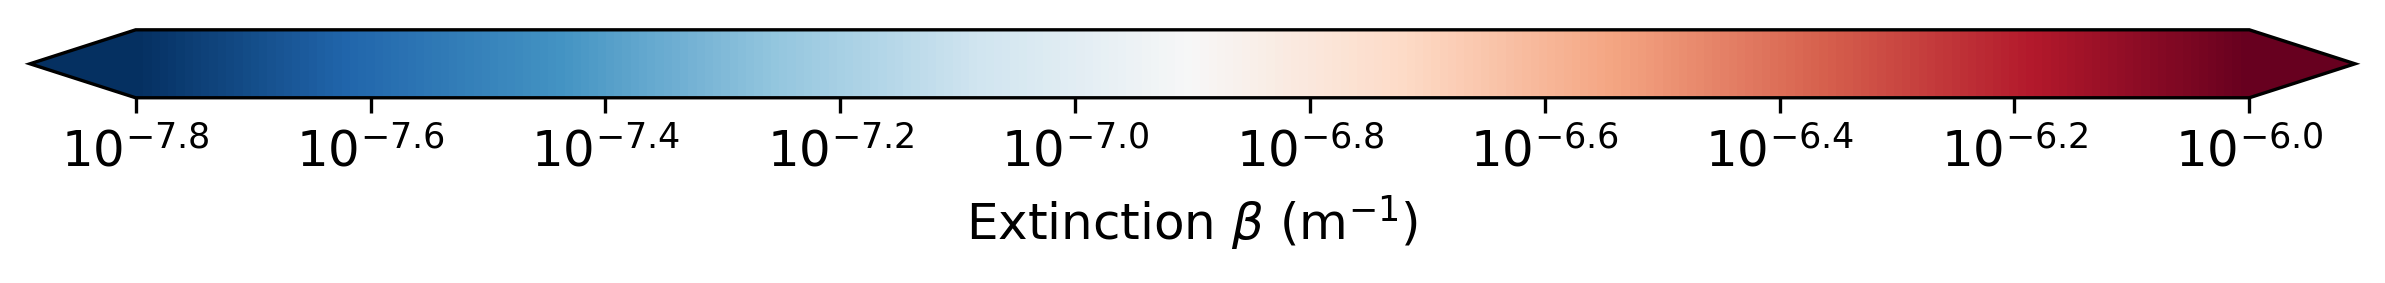
\includegraphics[width=.5\textwidth]{Fig/Extinction_colorbar}
\caption{Same as the figure~\ref{fig:dhl_2004_2008} for 8 images taken between 2008 and 2012
($L_s=\ang{340}-\ang{30}$) showing the drop and disappearance of the DHL.
The color schema is identical to the figure~\ref{fig:dhl_2004_2008} to provide
direct comparisons. In this case, the altitude range is extended down to 300 km
(where the model is less reliable).}
\label{fig:dhl_2008_2012}
\end{figure*}

As for the main haze, the detached haze collapses first in the Southern hemisphere, from 500 km to 425 km, and
then at the equator and in the northern hemisphere (Fig.~\ref{fig:dhl_2008_2012}c).
This is associated with the circulation turnover affecting first the summer hemisphere ascending branch.
With time, the detached haze gradually settled in altitude and finally disappear below 300 km.
Later ISS observations made with the Blue and Green filters visually show that the main DHL continues
its descend below 300 km during 2011. Since our current model was only tested for UV observations, we were not able
to observe its merge with main haze.
The complete collapse of the detached haze, as it appeared in the UV3 filter, is displayed in Fig.~\ref{fig:dhl_2008_2012}c to
Fig.~\ref{fig:dhl_2008_2012}h. We note that the column extinction is smaller at equator than at
other latitudes, and this is the case during entire period of the collapse.

During the fall, a second thin detached haze layer, at planetary scale, is evident above the collapsing detached
haze layer. In January 2010 (Fig.~\ref{fig:dhl_2008_2012}e), the detached haze layer was located between 375 and 400 km.
We can still see a double deck of haze, and this time the detached haze appears higher at the equator compared to the two
hemispheres, producing an arch. The haze peak extinction has globally increased by a factor of two due to sedimentation
in denser layers.

In August 2010 (Fig.~\ref{fig:dhl_2008_2012}f), one year after equinox, the detached haze layer continued
its drop down to 375 km around \ang{40}S and 400 km at the equator. It has gained in complexity with
multiple secondary layers up to 520 km. The detached haze formed a remarkable arch with a difference of about 50 km
in altitude between the equator and the poles as previously noticed by~\cite{West2011}.
This observation and the next one correspond to the same seasonal phase  of Voyager flybys ($L_s=\ang{8}$ and \ang{18}).
They can be compared directly.
We now know that this season was a time of rapid change, and that the Voyager probes observed transient situations.
Voyager also observed the detached haze higher near equator than elsewhere \citep{Rages1983, Rannou2000}.

Due to orbital constraints and mission planning, the next observation was made in September 2011
(Fig.~\ref{fig:dhl_2008_2012}g). The detached haze layer was, at that time, well below the level of the polar hoods.
Again, secondary detached layers show up as high as 470 and 520 km.

The south polar hood was not present in August 2010 (Fig.~\ref{fig:dhl_2008_2012}f) and appeared in less than 13 months.
This indicates that the circulation started to reverse around the equinox and the southward circulation sent haze to
the southern polar region and produced a polar hood. The change in haze distribution
is a very good indication of the timing of the equinoctial circulation turnover, as  discussed later. We note
that the strong haze depletion at 300 km and between \ang{30}S and \ang{20}N is real \change{(and visible in the I/F profiles)} but may be exaggerated at \ang{20}N
due to the limit of the retrieval procedure. At this altitude level, Titan's atmosphere is opaque to UV radiation
(see Fig.~\ref{fig:model_uncertainties}) and does not allow us to follow the main depletion below this altitude.

The last UV3 image we have showing a detached haze layer was taken in February of 2012 (Fig.~\ref{fig:dhl_2008_2012}h). At that
time, the initial detached haze had completely disappeared and the secondary detached haze layer was still descending
and had reached 400 km altitude. The secondary detached haze layer is not well delineated by a layer strongly depleted in aerosols.
The south polar hood increased its latitudinal extent northward to \ang{50}S and became larger than the northern
polar hood which tends to retreat.
